\chapter{Experiments}
\label{ch:testing}
I wrote all testing scripts and auxiliary functions in Python programming language. The scripts were written as Jupyter Notebook environment and saved in the corresponding file format \texttt{.ipynb}, lately these notebooks were saved as \texttt{.py} Python scripts. The set of utility functions is located in a file called \texttt{utils.py}. All experiments were run within Google Colaboratory\footnote{Google Colaboratory (Colab for short) is an product from Google Research. It allow Google users to write and execute python code within a web browser using a remote computer and its computing power. In the free version of Colab the computational resources are limited and vary over time due to the demands of other users. The product is available at \url{https://colab.research.google.com/}.} which provides a 12 GB RAM and a GPU Nvidia K80 with 12 GB memory.

In the experiments I chose three methods to be tested, namely, Tesseract, EasyOCR and keras-ocr. Each of them has corresponding Python package. For Tesseract I tried two approaches, one with pure Tesseract and another with CRAFT detection tool followed by Tesseract recognizer. I used four datasets that are described below in the following section. The three freely available datasets were chosen as representatives of OCR datasets.

\section{Datasets}
\label{sec:expDatasets}

\subsection{SCUT-CTW1500 dataset}

SCUT-CTW1500 dataset contains exactly 1500 images of real-world, scene text in English language. Sample images can be seen in Figure \ref*{Im:Dctw}. The key feature of this dataset is that each image contains horizontally aligned text, multioriented text and curved text. There are cases where the curvature is only slight and cases where text forms a circle with letter upside down. Recognizing multi-oriented and curved text is more of a challenge than pure horizontal text. This dataset is split to train and test data. Two thirds of dataset thus one thousand images for training and five hundred for testing. According to the description of this dataset on relevant GitHub repository dataset was manually labeled and lately corrected, therefore labels seem to be very accurate. However for example ground truth for image 1313.jpg misses all occurences of letter I, as the depicted font was probably misread.\cite{ctw,ctw2}

The ground truth for train data are in XML format and each file carries information about the file name of respective image file, text information -- i.e., words in a text line, 14 coordinates of a bounding polygon and coordinates, height and width of a circumscribed rectangle. Later the authors added coordinates of center point of each English letter to be used as detection ground truth. The ground truth of test data is in simple text file (TXT) and contains only 14 coordinates of the bounding polygon and a text which is within that region. There is a minor issue with labels that it usually contains a full text line with multiple words and coordinates are not assigned to individual words but to text region as whole. Most end-to-end system detect words rather than groups of corresponding words. This fact needs to be taken into account when evaluating results.

\begin{figure}[hbtp]
    \centering
    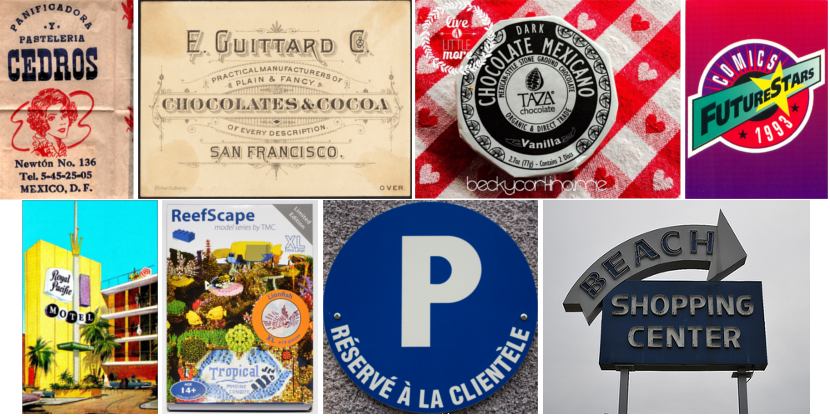
\includegraphics[scale=0.4]{obrazky/Dataset_ctw.png}
    \caption{Sample images of SCUT-CTW1500 dataset.}
    \label{Im:Dctw}
\end{figure}

\subsection{KAIST Scene Text Database}

This dataset contains 3000 images of photographed text. It can be divided into three major categories -- text of Korean language, English language and mixed languages. As I concentrate on text in latin script in this paper further information relates to the English language dataset. The number of images is then reduced to less than four hundred images. Figure \ref*{Im:Dkaist} shows few samples of this dataset. Photographed objects are mostly shop banners or parts of magazine front pages. Photographs were either taken by a high-resolution digital camera or a low-resolution mobile phone camera.\cite{kaist} Each photography has a ground truth description and a bitmap image. In the bitmap file only text is highlighted (by white or red color) and everything else apart from text is set as black. Ground truth files are in XML format and includes a name of an image, its resolution and bounding box for each word and also a bounding box for each letter of the word.

To use this dataset for testing and training the XML ground truth needed to be converted to string and int values. I wrote a parser, that combines letters to form a word that is within a given bounding box. I changed the notation of bounding boxes from one coordinate, width and height attributes to two top left and bottom right coordinates. The name of the parsing function is \texttt{read\_gt\_kaist}.

Unfortunately this dataset has few errors in filenames of corresponding files or in the content of XML files. Usually these are only typos, however they prevent automatic preprocessing of dataset. Due to this problem these mistakes need to be found and  manually corrected. Also there is a small number of ground truth XML file with fully missing data. 
Despite these shortcomings this dataset is useful because of the bitmap files. This allows to compare results of both images affected by shooting conditions and images dependent only on font and position.

\begin{figure}[hbtp]
    \centering
    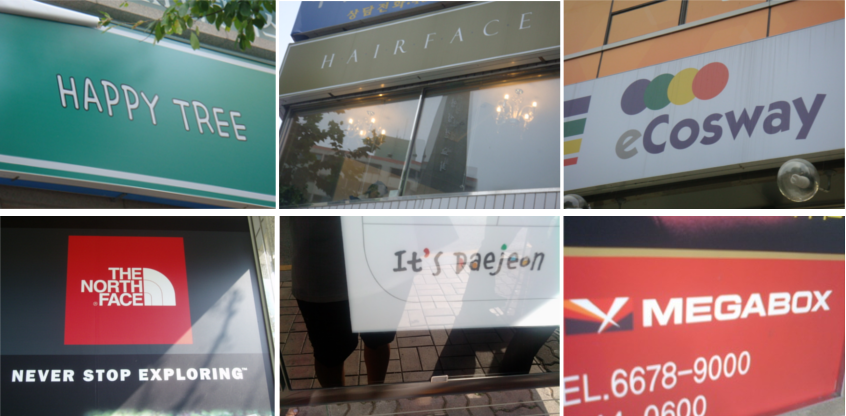
\includegraphics[scale=0.4]{obrazky/Dataset_kaist.png}
    \caption{Sample images of KAIST Scene Text Database dataset.}
    \label{Im:Dkaist}
\end{figure}

\subsection{Born-Digital Images}

Born-Digital Images contains data of images with text that can be found on various websites. Samples of this dataset can be found is in Figure \ref*{Im:Dbd}. There are mostly advertisements, company logos or website headers. Such pictures cannot be classified neither as real scene dataset, neither as synthetic one. On one hand  this dataset shares with scene datasets the variability in font styles and sizes, different text orientations and complex colour placement. On the other hand it differs in size because low resolution is significant in smooth and fast loading on websites. Also no noise is present due to lighting conditions. Geometrical deformations that result when capturing a real scene with camera also do not appear here. However compression to lower resolution can lead to artifacts and aliasing. In general we can say that letters are more clearly visible than in photographed text as easy readability is crucial in successful advertising.\cite{born-digital1}

The dataset is available for download from the website of Robust Reading Competition. First version was published in 2011 and revised two years later, it contains separate dataset for text localization, segmentation and then for word recognition. In 2015 they published an end-to-end dataset with ground truth for all tasks. The dataset is split in training and testing data. However, ground truth for testing data contains only a possible vocabulary of words in images and no coordinates. This might be due to the fact that the competition might be still ongoing or there was not a sufficient demand for complete ground truth. As for training data, each image has a corresponding TXT file with coordinates of four vertices of bounding rectangle and a word. Text lines are separated and the text within rectangle is always one word. Extracting ground truth is done in the function \texttt{read\_gt\_bd} and unlike preceding datasets there was no parsing needed, only read the desired values from a file. Unfortunately, there are quite a few missing words, usually words that have two or less characters. This can affect the evaluation when the model finds such a short, missing word.\cite{born-digital1}

\begin{figure}[hbtp]
    \centering
    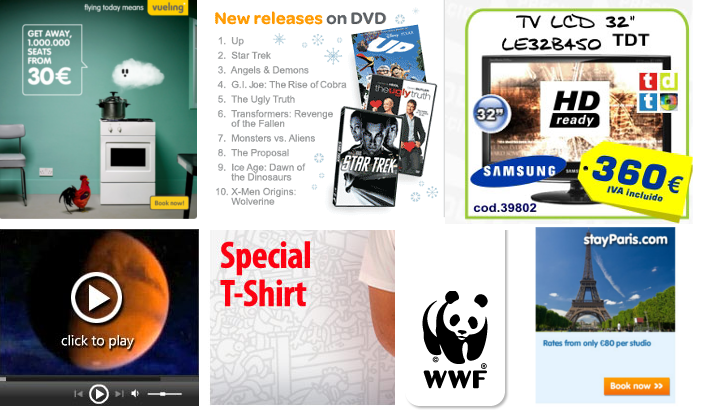
\includegraphics[scale=0.4]{obrazky/Dataset_born-digital.png}
    \caption{Sample images of Born-Digital Images dataset.}
    \label{Im:Dbd}
\end{figure}


\subsection{Vienna City Poster Dataset}

The Vienna City Library possesses a collection of 350,000 poster images. A sample of the collection was provided by the organization to the Technical University of Vienna for research purposes. It consists of 5050 images. From these images we manually labeled 257 images and created a testing dataset. Sample of the dataset is in Figure \ref*{Im:Dvienna}. As it can be seen from the example images, the dataset includes mainly posters with German language, though few images have words in English or Czech.

\begin{figure}[hbtp]
    \centering
    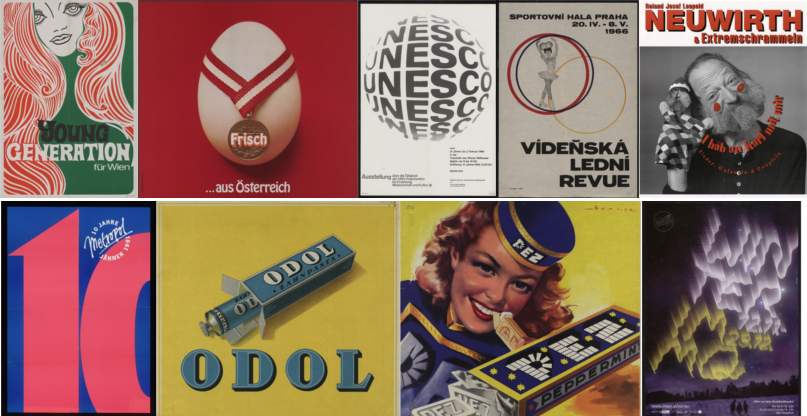
\includegraphics[scale=0.5]{obrazky/Dataset_vienna.png}
    \caption{Sample images of Vienna City Poster Dataset.}
    \label{Im:Dvienna}
\end{figure}


The posters have neither the characteristic of a scanned text documents, neither of scene images. They are most similar to born digital images. However for the posters is typical one thing -- a part of the text is large relative to the image size and another part is tiny. The huge text is usually a brand or product name or a name of an event. The small text is the name of the author of the poster or the printer where the posters was printed. Both of these texts are a challenge for an OCR engine, because large letters are misinterpreted as objects and the height of the tiny ones is not bigger then twenty pixels and letters are often blurred. Middle-sized text also appears in the posters and is generally well recognized.

Due to the presence of the small text. All images in the dataset need  to be in the original resolution. The bigger side is always 4096 pixels. This leads to a large dataset even when the number of images is less then three hundred. A single JPG image has approximately 4 Megabytes. A PNG image in the dataset has about 20 Megabytes. To reduce the final size of the dataset I decided to convert the PNG files to JPG\footnote{For converting the images I used the console application ImageMagick, with the command \newline \tn{for f in *.png ; do convert "\$f" "../alljpg/\$\{f\%.*\}.jpg" ; done}.}. The final dataset of JPG images is 1.1 GB large, before it was 2.8 GB. The high resolution of images makes demands on the hardware when working with the dataset and makes it impossible to run on machines with insufficiently large computing memory.

The annotation tool used for labeling the selected posters is called Aletheia from the PRiMA Research\footnote{More information available at https://www.primaresearch.org/tools/Aletheia}. The program can be downloaded for Windows operating system, it offers both Lite and Pro version. A free one month trial is offered or for academic use the PRiMA Research gives an extended license. Using this tool we labeled every separate word or group of letters (such as poster identification number) found in an image on the selected posters. Words that were forming a text line, were afterwards labeled as a text line (single word is a text line consisting of one word). Individual characters were not labeled. Bounding boxes for both words and text lines are rectangles, even for curved text. Word bounding boxes were drawn pixel precise with the intention of no margin between the box and the word. Aletheia software produces a XML file with PRiMA Research tags, example for the image P-2151.jpg is in the code below. 

\begin{lstlisting}[label=lst:xml]
<?xml version="1.0" encoding="UTF-8"?>
<PcGts xmlns="http://schema.primaresearch.org/PAGE/gts/pagecontent/2019-07-15" xmlns:xsi="http://www.w3.org/2001/XMLSchema-instance" xsi:schemaLocation="http://schema.primaresearch.org/PAGE/gts/pagecontent/2019-07-15 http://schema.primaresearch.org/PAGE/gts/pagecontent/2019-07-15/pagecontent.xsd">
<Creator></Creator>
<Created>2022-03-14T11:42:27</Created>
<LastChange>2022-03-14T11:42:27</LastChange></Metadata>
<Page imageFilename="P-2151.jpg" imageWidth="2524" imageHeight="4096">
<TextRegion id="tempReg357564684568544579089">
<Coords points="0,0 1,0 1,1 0,1"/>
<TextLine id="l4">
<Coords points="264,2496 264,2810 2301,2810 2301,2496"/>
<Word id="w10">
<Coords points="264,2496 264,2810 2301,2810 2301,2496"/>
<TextEquiv>
<Unicode>GENERATION</Unicode></TextEquiv></Word>
<TextEquiv>
<Unicode>GENERATION</Unicode></TextEquiv></TextLine>
...
\end{lstlisting}









\section{Results}



I have split the experiments by the four datasets and made comparisons. Prediction methods were examined with a different setting of parameters where possible.

The pipeline of each testing script is as follows.
\begin{enumerate}
    \item Installation of packages that are not in the default Google Colab setting.
    \item Importing dependencies for the project including custom utility functions from \texttt{utils.py}.
    \item Google Drive of the user that runs Google Colab is mounted. (Authentication is needed)
    \item Image files and ground truth files are loaded. Ground truth is converted from files to tuple of string and integer coordinates.
    \item If desired a short preprocessing of images is done (grayscale, Otsu thresholding).
    \item Setup of parameters for OCR.
    \item Model loading.
    \item Prediction.
    \item Conversion of prediction to a unified format (List of tuples of string and integer coordinates for each image, then joined to a list, which contains prediction for all images.)
    \item Computation of evaluation metrics IOU an CER.
    \item Saving and visualizing results.
\end{enumerate}

Next I will shortly described possible setups of each of the three methods I used in the experiments. It will be  followed by discussion of the results of test divided into sections by the four datasets.

\subsection*{EasyOCR}
I used the version 1.5.0 of the EasyOCR python package. The experiments were run using a GPU. I used two different settings for EasyOCR engine -- the basic one which tends to detect and recognize text as single word objects and the second setting merges close words together creating text lines of words that belong together.

\subsection*{Keras-OCR}
The keras\_ocr-0.9.1 package for Python was used in experiments. It was necessary to compute the predictions on GPU, due to the limited GPU on Google Colab and the size of the images needed to be processed one by one although Keras allows to process images in batches. Keras-OCR predictions are case insensitive, because the default model does not support uppercase letters. I trained the Keras recognition model on SCUT-CTW1500 dataset (on the one thousand training images), first a trained the default model with lower case alphabet, then with the same alphabet and a space character and finally with uppercase letters and a set of special characters. In the results discussion it will be shown that after training the model does not offer better results than the original model. THe original model is already very successful and was well trained on much larger datasets.

Each of the training took about an hour on Google Colab GPU. I set 100 epochs and an early stopping based on the value of validation loss. The validation data were taken from the train data as 20\% of the whole training part. First the I used early stopping after 10 non decreasing values, then after 30, but in both cases the model could not get any better than 14\% validation loss.

% graph

\subsection*{Tesseract}
The version of Tesseract installed on Google Colab is tesseract 4.0.0-beta.1 with leptonica-1.75.3, which means that the LSTM network is available. For testing I used the OCR Engine mode (OEM) 3, that is Legacy + LSTM engines. As for Page segmentation modes (PSM) I used numbers 3, 4, 6, 8 and 11, which are "Fully automatic page segmentation, but no OSD. (Default)", "Assume a single column of text of variable sizes.",  "Assume a single uniform block of text.",  "Treat the image as a single word." and "Sparse text. Find as much text as possible in no particular order." respectively. I used PSM 3 only initially and dropped it beacuse prediction was strongly inefficient, so it is not included in result statistics. PSM 8 was used for testing Tesseract with CRAFT, because CRAFT crops an image into segments where there is only one word (or a short text line), therefore Tesseract needed to treat the image as a single word. The rest of mentioned PSMs were applied for examining the behavior of pure Tesseract engine. 




\subsection*{Born-Digital}

First, the Born-Digital Images dataset was tested with images in predictions and ground truth were set to be in lowercase and all special characters except for space were removed. There were 13 different testing runs with three tested methods.  In Figure \ref*{Im:resBD} are the results of this testing and in Table \ref*{Tab:resBD} is corresponding information about each run. 

The best CER value was achieved by tuned EasyOCR engine, where no split was done on predicted text (letter D in Fig. \ref*{Im:resBD}). We can see from the graph and table, that EasyOCR and keras-OCR had significantly better results than Tesseract. Also it can be said that tuning of EasyOCR model results in higher both IOU and CER of approximately 20\% more than with basic EasyOCR setup of parameters. Keras-OCR performs simlarly with split and no split option and in both cases gives satisfactory results.

When we compare Tesseract with its own detection model and Tesseract with CRAFT tool, we can see that CRAFT increases the CER metric by more than 12\%, however the IOU metric fluctuates for all cases around 50\%. Whether the image is in RGB color scheme or in grayscale has only a little impact on the results, generally it differed only by about 2\%. Same minor difference is when split or no split option is set. If the Otsu thresholding was performed and the image was then binarized, results were worse than when Tesseract itself performs the binarization. Better results were when PSM tesseract parameter was set to 11 rather then PSM 4.

{
\begin{figure}[hbt!]
    \centering
    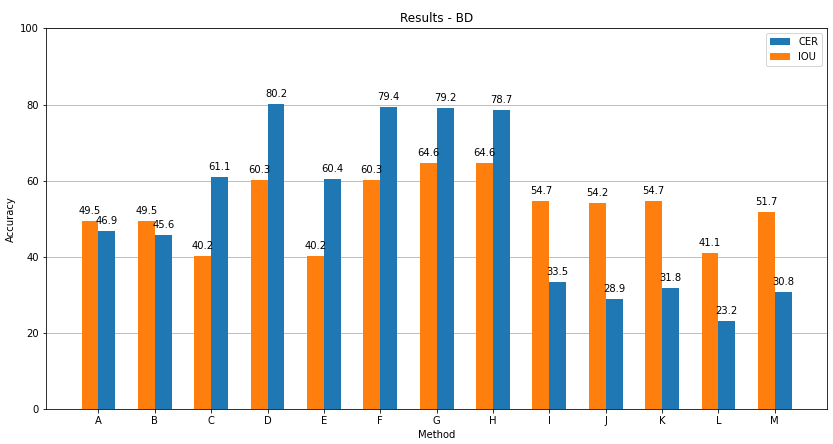
\includegraphics[scale=0.5]{obrazky/grafy/resBD.png}
    \caption{Results of experiments performed on Born-Digital Images dataset. Information about each method is in Table \ref*{Tab:resBD}.}
    \label{Im:resBD}
\end{figure}
\begin{table}[!hbt]
    \centering
    \begin{tabular}{|l|l|l|}
    \hline
        Key & Method & Properties \\ \hline
        A & tesseract+CRAFT &  no split, psm8\\ 
        B & tesseract+CRAFT &  split, psm8\\ \hline
        C & easyOCR &  no split, no tuning\\ 
        D & easyOCR &  no split, tuning\\ 
        E & easyOCR &  split, no tuning\\ 
        F & easyOCR &  split, tuning\\ \hline
        G & keras-OCR &  no split\\ 
        H & keras-OCR &  split\\ \hline
        I & tesseract & colored, no split, psm11\\ 
        J & tesseract & binary, split, psm11\\ 
        K & tesseract & colored, split, psm11\\ 
        L & tesseract & binary, split, psm4\\ 
        M & tesseract & colored, split, psm4\\ \hline
    \end{tabular}
    \caption{A table of keys for methods and parameters of experiments performed on Born-Digital Images dataset for Figure \ref*{Im:resBD}.}
    \label{Tab:resBD}
\end{table}
}

Next I performed tests with case sensitive option and with special characters included.

\subsection*{SCUT-CTW1500 dataset}
The SCUT-CTW1500 dataset was again first tested with predictions and ground truth were set to be in lowercase and all special characters except for space were removed. 14 different testing were run.  In Figure \ref*{Im:resCTW} are the results of the testing and the corresponding information about each run is in Table \ref*{Tab:resCTW}. 

This time the best CER value ($76.4\%$) was achieved by keras-OCR model, where split was performed on predicted text (letter H in Fig. \ref*{Im:resCTW}). It can be seen from the graph and table, that EasyOCR and keras-OCR had again significantly better results than Tesseract. In testing of CTW1500 dataset this time keras-OCR generally performed better than EasyOCR in CER metric by roughly 10\%. The tuning of EasyOCR model results in lower both IOU and CER of approximately 2\% less than with basic EasyOCR setup of parameters. This might by probably due to the fact that EasyOCR model was trained on data similar to CTW1500 dataset rather then Born-Digital Images dataset Keras-OCR performs simlarly with split and no split option and in both cases gives satisfactory results.

The Comparison of Tesseract with its own detection model and Tesseract with CRAFT tool shows that with CRAFT the CER metric increased by almost than 20\% as well as the IOU metric that increased by more than 30\%. Plain Tesseract results are again the worst and are not heavily influenced by color scheme or slight scaling changes. 

\begin{figure}[hbt!]
    \centering
    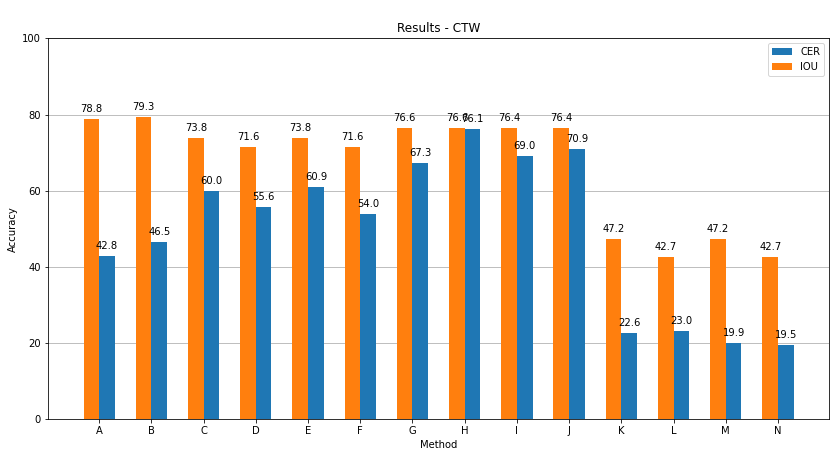
\includegraphics[scale=0.5]{obrazky/grafy/resCTW.png}
    \caption{Results of experiments performed on CTW dataset. Information about each method is in Table \ref*{Tab:resCTW}.}
    \label{Im:resCTW}
\end{figure}
\begin{table}[!ht]
    \centering
    \begin{tabular}{|l|l|l|}
    \hline
        Key & Method & Properties \\ \hline
        A & tesseract+CRAFT & no split \\ 
        B & tesseract+CRAFT & split \\ \hline
        C & easyOCR & nosplit, notuning \\ 
        D & easyOCR & no split, tuning \\ 
        E & easyOCR & split, notuning \\ 
        F & easyOCR & split, tuning \\ \hline
        G & keras-OCR & original image width, no split \\ 
        H & keras-OCR & original image width, split \\ 
        I & keras-OCR & original image width, split, trained spaces \\ 
        J & keras-OCR & original image width, split, trained \\ \hline
        K & tesseract & 3000px image width, no split \\ 
        L & tesseract & color, no split, psm11 \\ 
        M & tesseract & split, psm11\\ 
        N & tesseract & color, split, psm11 \\ \hline
    \end{tabular}
    \caption{A table of keys for methods and parameters of experiments performed on SCUT-CTW1500 dataset for Figure \ref*{Im:resCTW}.}
    \label{Tab:resCTW}
\end{table}

\subsection*{KAIST Scene Text Database}

Testing of performance of the three methods on KAIST dataset with case insensitivity and no special characters was done in 22 different runs. Eight of them were on KAIST bitmap images, as these images do not have a misleading background the results are significantly better than on original photographes. The results can be seen in Figure \ref*{Im:resK} and the corresponding information is in Table \ref*{Tab:resK}. 
The best results on the bitmap images part of KAIST dataset were performed by EasyOCR dataset with no splitting and CER value is $82.2\%$ high (letter B in Fig. \ref*{Im:resK}). This method with the same setup is also best with KAIST dataset unedited photographs. Due to the character of the dataset for all cases the no split option is distinctly better. 

Keras-OCR had slightly lower values of CER than EasyOCR and IOU values are even lower by generally 15\%. Still it is by 20\% higher than results of plain Tesseract and comparable with Tesseract and CRAFT combination. Tesseract had this time best but still way too low results with PSM 6. PSM 4 led to CER value as low as 18\%. Color scheme did not have a distinguishable impact on the results.
 
\begin{figure}[hbt!]
    \centering
    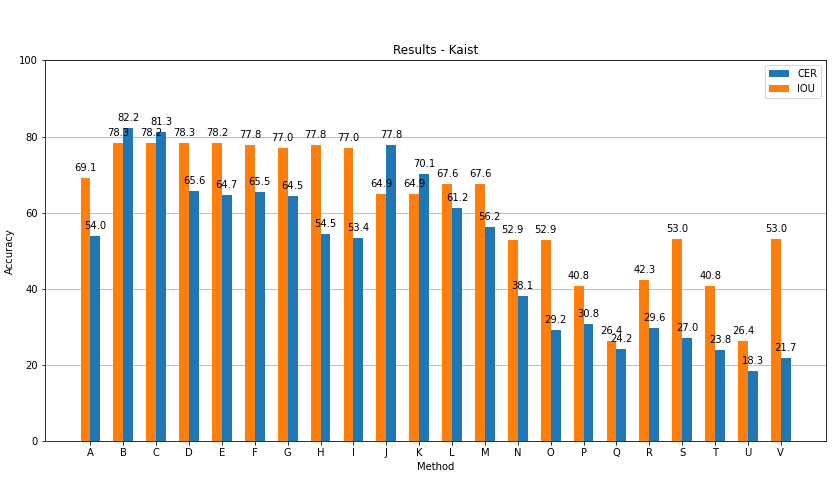
\includegraphics[scale=0.5]{obrazky/grafy/resKaist.png}
    \caption{Results of experiments performed on KAIST Scene Text Database. Information about each method is in Table \ref*{Tab:resK}.}
    \label{Im:resK}
\end{figure}
\begin{table}[!ht]
    \centering
    \begin{tabular}{|l|l|l|}
    \hline
        Key & Method & Properties \\ \hline
        A & tesseract+CRAFT & no split \\ \hline
        B & easyOCR & bmp, no split, no tuning \\ 
        C & easyOCR & bmp, no split, tuning \\ 
        D & easyOCR & bmp, split, no tuning \\ 
        E & easyOCR & bmp, split, tuning \\ 
        F & easyOCR & no split, no tuning \\ 
        G & easyOCR & no split, tuning \\ 
        H & easyOCR & split, no tuning \\ 
        I & easyOCR & split, tuning \\ \hline
        J & keras-OCR & bmp, no split \\ 
        K & keras-OCR & bmp, split \\ 
        L & keras-OCR & no split \\ 
        M & keras-OCR & split \\ \hline
        N & tesseract & bmp, no split, psm11 \\ 
        O & tesseract & bmp, split, psm11 \\ 
        P & tesseract & colored, no split, psm11 \\ 
        Q & tesseract & colored, no split, psm4 \\ 
        R & tesseract & colored, no split, psm6 \\ 
        S & tesseract & no split, psm11 \\ 
        T & tesseract & colored, split, psm11 \\ 
        U & tesseract & colored, split, psm4 \\ 
        V & tesseract & split, psm11 \\ \hline
    \end{tabular}
    \caption{A table of keys for methods and parameters of experiments performed on KAIST Scene Text Database for Figure \ref*{Im:resK}.}
    \label{Tab:resK}
\end{table}



% Training took one hour and stopped after 57 epochs ,10.979148864746094,20.5778751373291. Continued training.

% trained no spaces 
% [[('bruno', 'brung', 0.2)],
%  [('optique', 'ortinu', 0.42857142857142855),
%   ('optique', 't', 0.8571428571428571)],
%  [('promotion', 'mgtioa', 0.5555555555555556),
%   ('promotion', 'rro', 0.7777777777777778)],
%  [('la', 'bne', 1.0),              ('paire', 'paite', 0.2)]]
%  [[('panns', 'aine', 0.6)],
%  [('1958', '1953', 0.25), ('since', 'simce', 0.2)],
%  [('food', 'food', 0.0), ('real', 'rea', 0.25)]]
%   ('la', 'loz', 0.6666666666666666),
%                 ('paire', 'paite', 0.2)]]
%                 [[('panns', 'aine', 0.6)],
%                 [('1958', '1953', 0.25), ('since', 'simce', 0.2)],
%                 [('food', 'food', 0.0), ('real', 'rea', 0.25)]]


% CTW
% training with special chars case insensitive no special split
% [[('bruno', 'bruns', 0.2)],
%  [('optique', 'optoue', 0.2857142857142857), ('optique', 'srss', 1.0)],
%  [('promotion', 'bre', 0.8888888888888888),
%   ('promotion', 'motion', 0.3333333333333333)],
%  [('2eme', 'enne', 0.75), ('la', 'le', 0.5), ('la', 'salls', 0.8)]]

%  s no splitem 60 to je fakt malo ani ne v grafu

%  velka pismena a znaky
%  [[('BRUNO', 'BRUNS', 0.2)],
%  [('OPTIQUE', 'OPTOUE', 0.2857142857142857), ('OPTIQUE', 'SRSS', 1.0)],
%  [('PROMOTION', 'BRE', 0.8888888888888888),
%   ('PROMOTION', 'MOTION', 0.3333333333333333)],
%  [('2eme', 'enne', 0.75), ('La', 'Le', 0.5), ('La', 'Salls', 0.8)]]

%  [[('DOUGLASTON', 'BOUGLASTON', 0.1)],
%  [('E-313', 'E313', 0.2)],
%  [('L164', 'Lbl6w', 0.6)],
%  [('F.D.N.Y.', 'EDNY', 0.625)]]

% BD

% nula

% [[('flying', 'tying', 0.3333333333333333)],
%  [('today', 'todoy', 0.2)],
%  [('means', 'eons', 0.4)],
%  [('vueling', 'VUelnng', 0.42857142857142855)],
%  [('GET', 'GET', 0.0)],
%  [('', 'AVAY.', 1)],
%  [('1.000.000', '1.000.000', 0.0)],
%  [('SEATS', 'SEATS', 0.0)],
%  [('FROM', 'FRON', 0.25)],
%  [('30€', '303', 0.3333333333333333)],
%  [('Book', 'BOOK', 0.75)],
%  [('now!', 'nowi', 0.25)]]

Case sensitivity


when default model is used and special characters and case sensitivity of ground truth labels is observed CER accuracy reaches only less than thirty percent. 


\subsection*{Vienna}

easyocr tuning split
easyocr tuning split special char, sensitivity
easyocr tuning split no correction

easyocr tuning nosplit - better one deci
easyocr tuning no split special char, sensitivity - better

easyocr notuning split
easyocr notuning nosplit 
keras 15 minut easyocr 3 minuty


keras sensitivita a specila na nic pac to neumi 32procent